Some published numerical experiments have over time become benchmarks for other codes, while some 
others showcased comparisons between codes. Here is a short list of 'famous' benchmarks' in the 
computational geodynamics community.

\begin{itemize}
\item the plastic brick \cite{lemm08,kaus10,qurj09,mishin11,maie12,spmw16,gltf18,frbt19}
\item 2D Rayleigh-Benard convection (Blankenbach)  \cite{blbc89,trha98,chhl08,king09,lezh11,vyrc13,trab90,bepo10}
\item 2D Rayleigh-Taylor convection/instability \cite{pros81,trab90,wesc92,popo92,soga01,bast02,taki03,bomh06, basd08,qurj09,saev10,como97,lezh11,lomw12,vyrc13,vaks97,bomh06,chtl13,deka08,mishin11,maie12,fusc13,devv00a,dadh07,demh19}


\item 3D Rayleigh-Taylor instability \cite{fukk08,vosc15}
\item subduction problems \cite{scbe08,vack08,cehg14}
\item numerical sandbox \cite{bbeg06,maie12,busa16,gltf18}
\item the Stokes sphere \cite{galemanual}
\item the sinking block \cite{thie11,cehg14,gery10,geyu03,mamo08,mishin11,fumt11,maie12}
\item multiple sinkers \cite{mabl14,mabl15}
\item 2D compressible Stokes flow problem \cite{itki94,tagu07,lezh08,kilv10,lizh13}
\item 3D convection at infinite Prandtl number (Busse) \cite{bucc93,trha98}
\item Free surface evolution \cite{crsg12}
\item Love's problem \cite{bebe04}
\item Poiseuille flow \cite{fojg94,fuku11}
\item Couette flow with temperature dependent viscosity \cite{egat10,demh19}
\item Couette flow with shear heating \cite{egat10}
\item Poiseuille-Couette flow \cite{fusc13}
\item Lid driven Cavity \cite{foth79,ghgs82,bope98,kawa61}
\item Wannier flow \cite{wann50,yemu99}
\item bending of elastic plate/beam \cite{cehg14,boht08a,vosc15,egat10,demh19}
\item flexure of finite length elastic plate \cite{chtl13}
\item thermal diffusion of half-cooling space \cite{chtl13}
\item stress build-up in Maxwell visco-elastic material \cite{geyu07,chtl13,egat10,demh19}
\item plastic oedometer test  \cite{chtl13}
\item SolCx \cite{mamo08,demh19}
\item SolKz \cite{mamo08,demh19}
\item SolVi, inclusion \cite{kapo06,maie12,deka08,bepo10,vosc15,demh19}
\item channel flow (nonlinear) \cite{maie12,frbt19,gery10,egat10} (\bscthesis) \index{BSc Thesis}
\item indentor, punch problem \cite{engl82,thfb08,mota77,gepd98,gltf18}. See also \cite{hukm03,fojd04,gerb12} for application.
\item relaxation of sinusoidal topography \cite{crsg12,robh17}
\item single layer visco-elastic folding \cite{vosc15}
\item Three-dimensional folding of an embedded viscous layer in pure shear \cite{flet91}
\item dam-break problem \cite{moeb99,bacp07,liir07,lemx08,homa09,anco09,grdn97,hini81,basd08}
\item hot blob \cite{bugs09,fumt11}
\item visco-elastic flow past a cylinder in a channel \cite{bepo10}
\end{itemize}

\todo[inline]{go through my papers and add relevant ones here}

%..................................................
\subsubsection{Relaxation of sinusoidal topography}

Following Kramer et al. \cite[Section 3.1.1]{krwd12} and \cite{robh17} 
the benchmark consists of the relaxation of surface topography in a 
two-dimensional Cartesian box with an isoviscous fluid. 
Free slip boundary conditions are imposed on the sides and bottom of the domain.
The setup is as follows:

\begin{center}
\begin{minipage}{0.45\textwidth}
\centering
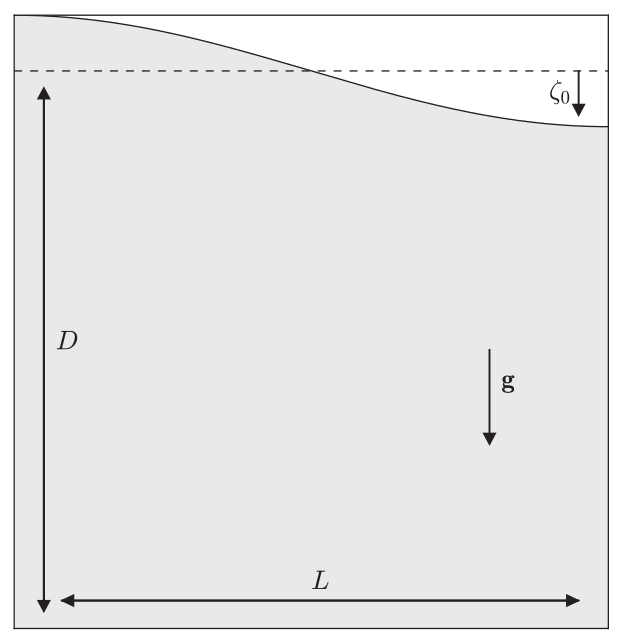
\includegraphics[height=0.8\textwidth]{images/benchmark_relaxation/robh17}\\
{\small Taken from \cite{robh17}. Setup for the free surface relaxation benchmark.
For the tests $\rho=\eta=g=L=D=1$ and $\xi_0=0.005$.}
\end{minipage}\hfill
\begin{minipage}{0.45\textwidth}
\centering
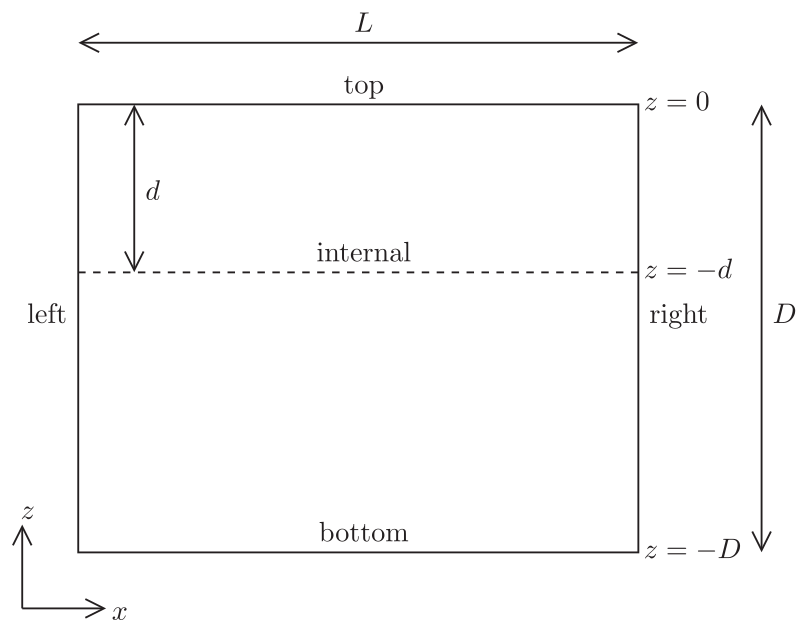
\includegraphics[height=0.8\textwidth]{images/benchmark_relaxation/krwd12}\\
{\small Taken from \cite{krwd12}. $D=3\cdot 10^6$,$\eta=10^{21}$, $\rho=4500$, $g=10$, $\xi_0=10^3$m, and 
$L=D/4,D/2,D,2D,4D$.}
\end{minipage}
\end{center}
and the infinitesimal sinusoidal perturbations to the free surface is given by
\[
\xi(x,t=0)=\xi_0 \cos \left( \frac{2 \pi n x}{L}  \right)
\]
where $n$ is a wavenumber which is an integer multiple of 1/2 (taken to be 1/2 exactly in both cases).


%...............................................................
\subsubsection{the plastic brick}

\Literature \cite{hans03,moml07,lemm08,kaus10,egat10,qurj09,mishin11,maie12,spmw16,gltf18,frbt19,aspectmanual}

Pretty much all of the brick-type (elasto-)visco-plastic experiments in the literature
introduce a weak seed at the bottom of the domain to seed deformation (the shear bands
will ultimately stem from it). 
Dimensioned and dimensionless experiments have been carried out, with or without 
elastic behaviour, with or without adaptive mesh refinement, with first order and 
second order quadrilateral elements or Taylor-Hood triangles, with or without 
Newton algorithm, in extension and compression, with or without time-stepping,
with or without viscous lower layer. 


\begin{center}
\begin{minipage}{0.45\textwidth}
\centering
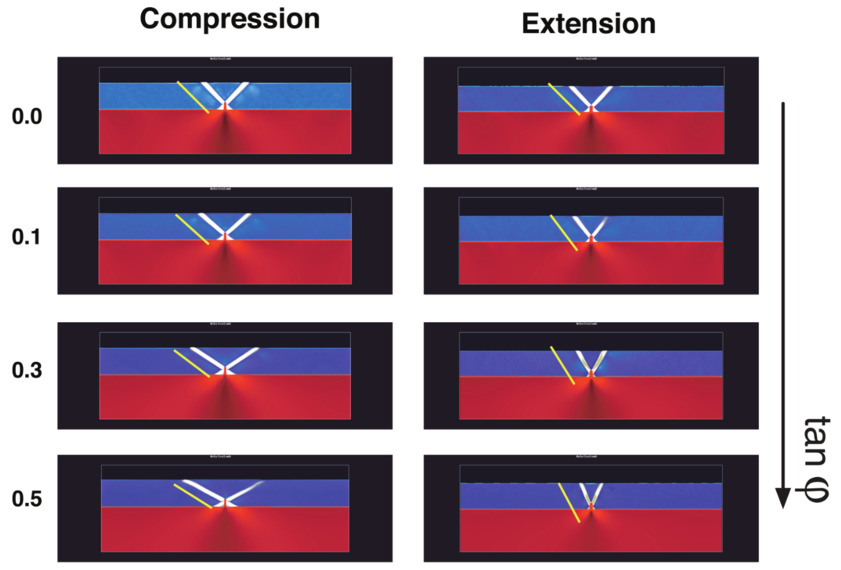
\includegraphics[height=0.8\textwidth]{images/benchmark_brick/moml07}\\
{\small Moresi et al, 2007 \cite{moml07}}
\end{minipage}\hfill
\begin{minipage}{0.45\textwidth}
\centering
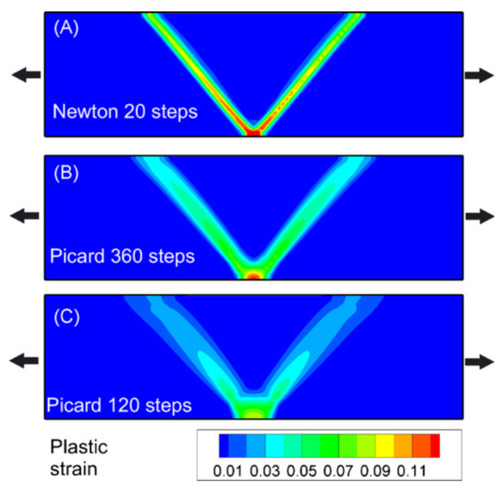
\includegraphics[height=0.8\textwidth]{images/benchmark_brick/poso08}\\
{\small Popov et al, 2008 \cite{poso08}}
\end{minipage}
\end{center}

\begin{center}\noindent\rule{8cm}{0.4pt}\end{center}

\begin{center}
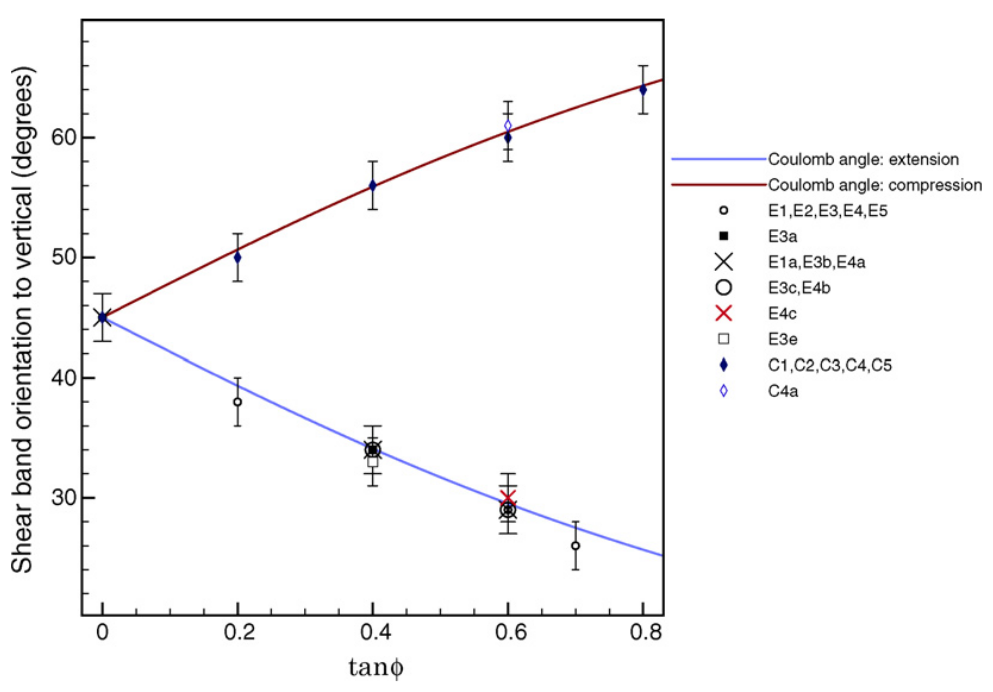
\includegraphics[width=5cm]{images/benchmark_brick/lemm08a}
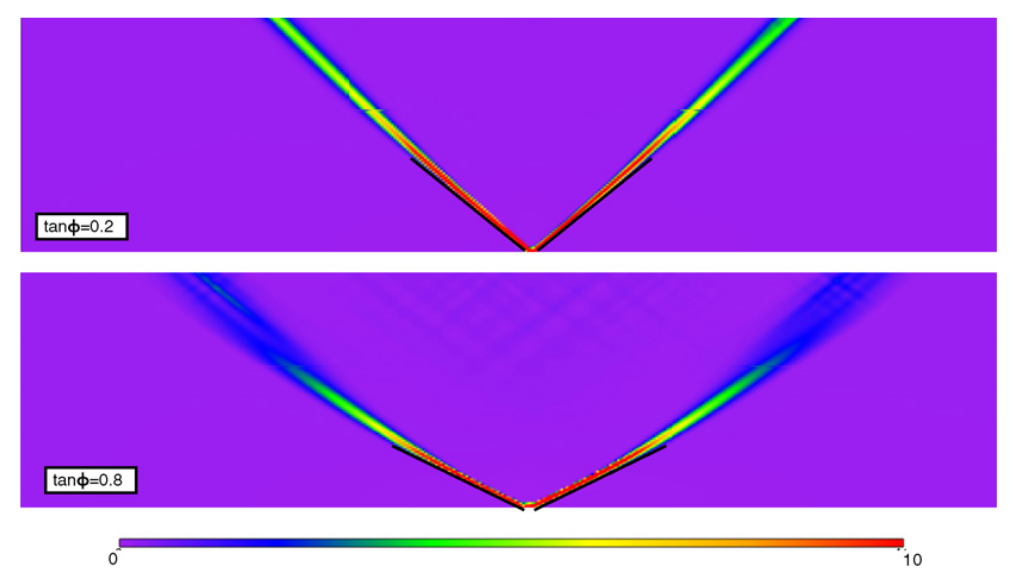
\includegraphics[width=5cm]{images/benchmark_brick/lemm08b}
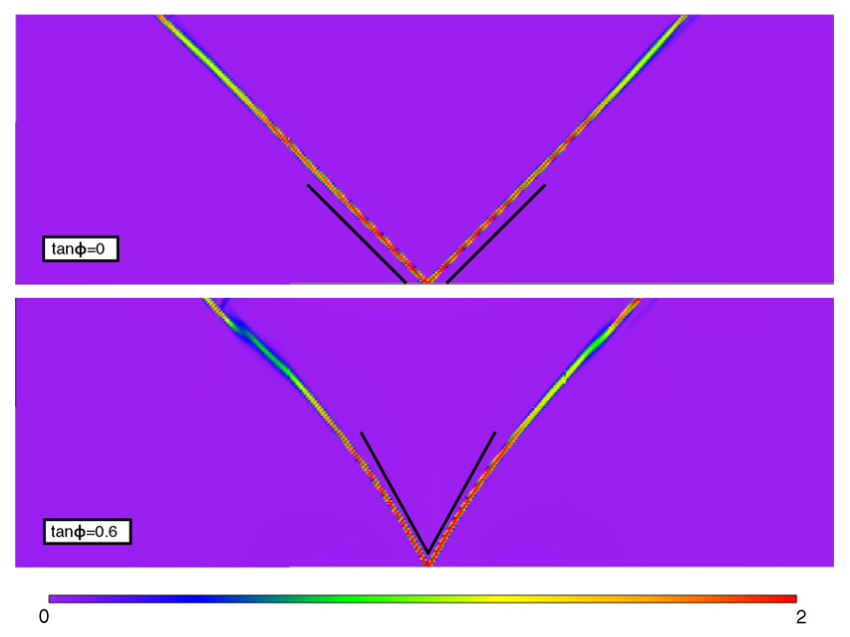
\includegraphics[width=5cm]{images/benchmark_brick/lemm08c}\\
{\small Lemiale et al, 2008 \cite{lemm08}}
\end{center}

\begin{center}\noindent\rule{8cm}{0.4pt}\end{center}

\begin{center}
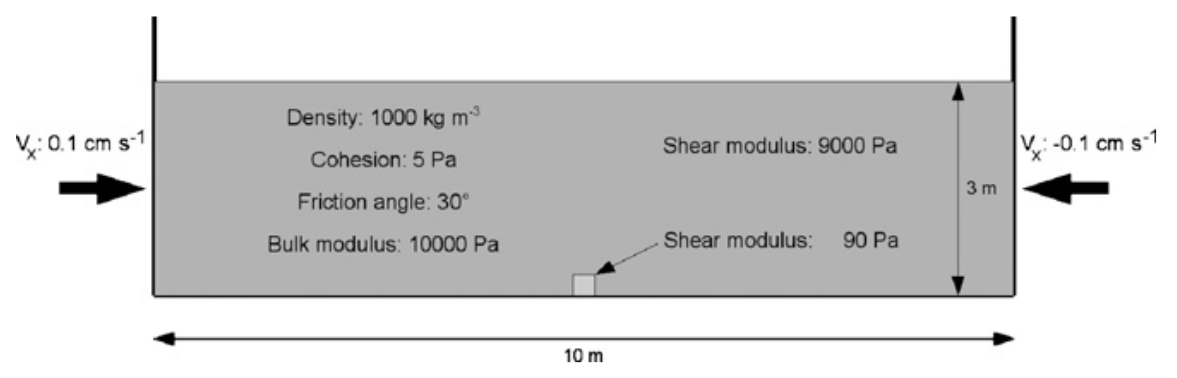
\includegraphics[width=7cm]{images/benchmark_brick/qurj09b}
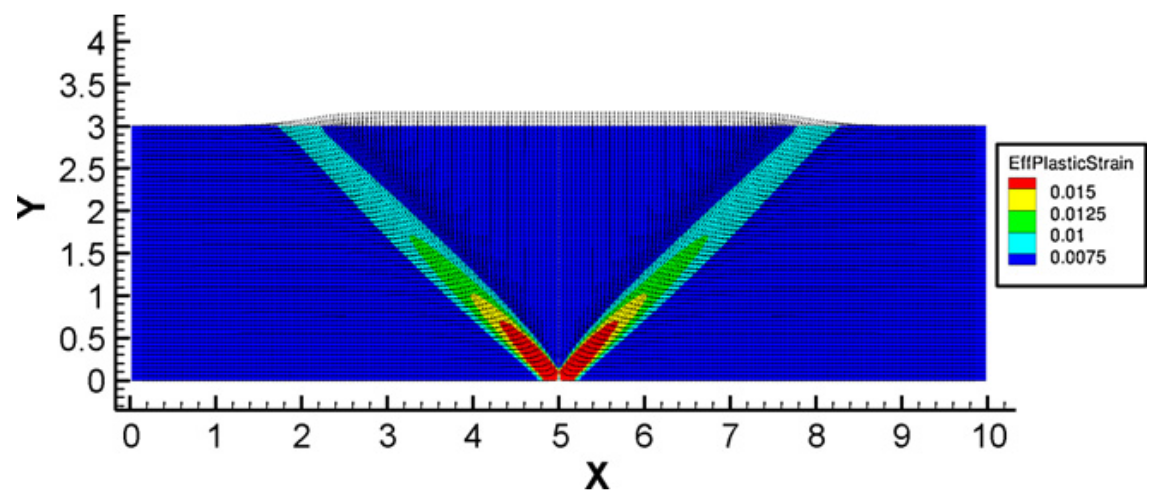
\includegraphics[width=6cm]{images/benchmark_brick/qurj09a}\\
{\small Quinteros et al., 2009 \cite{qurj09}}
\end{center}

\begin{center}\noindent\rule{8cm}{0.4pt}\end{center}

\begin{center}
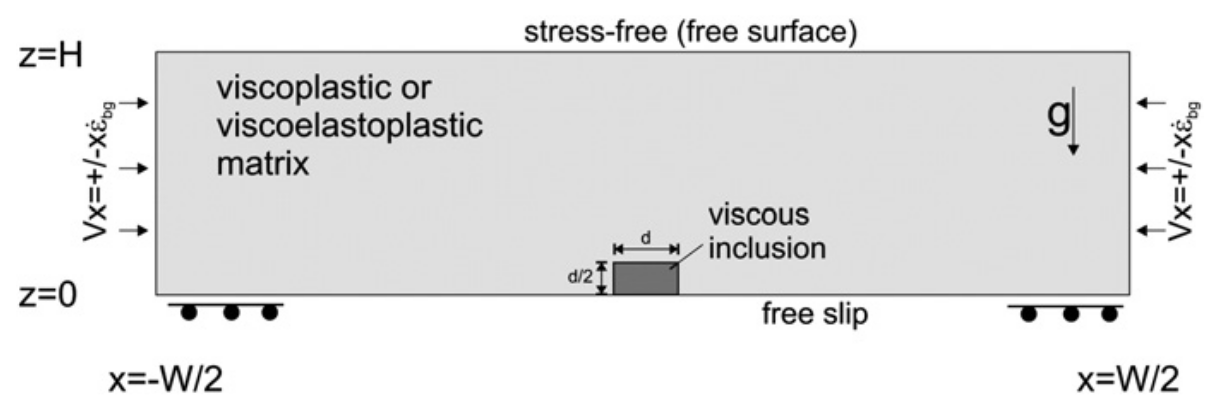
\includegraphics[width=5cm]{images/benchmark_brick/kaus10a}
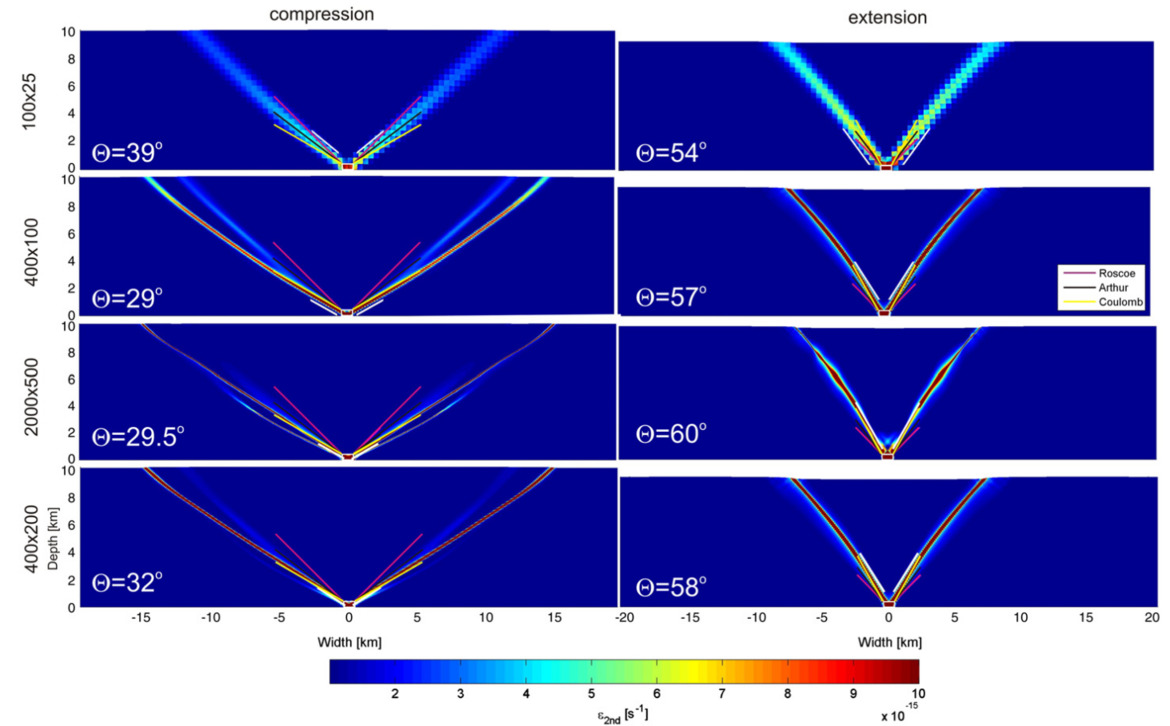
\includegraphics[width=5cm]{images/benchmark_brick/kaus10b}
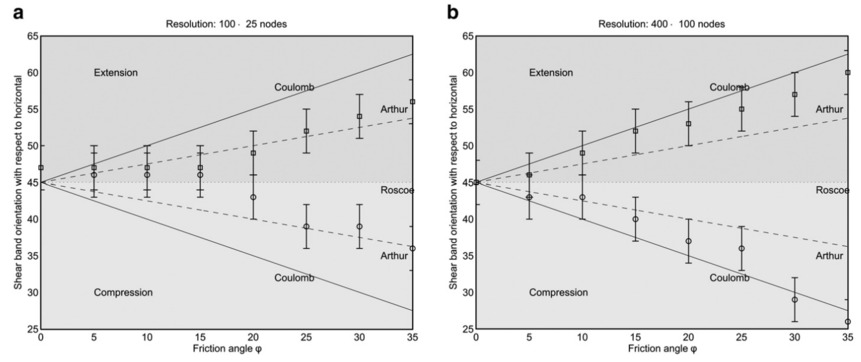
\includegraphics[width=5cm]{images/benchmark_brick/kaus10c}\\
{\small Kaus, 2010 \cite{kaus10}}
\end{center}

\begin{center}\noindent\rule{8cm}{0.4pt}\end{center}

\begin{center}
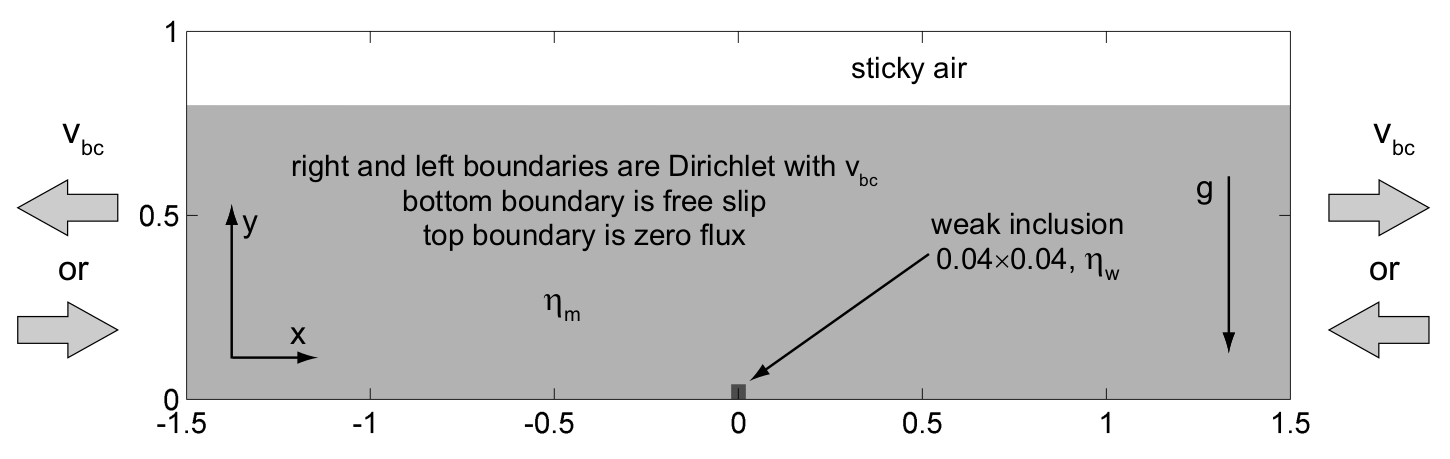
\includegraphics[width=3.74cm]{images/benchmark_brick/mishina}
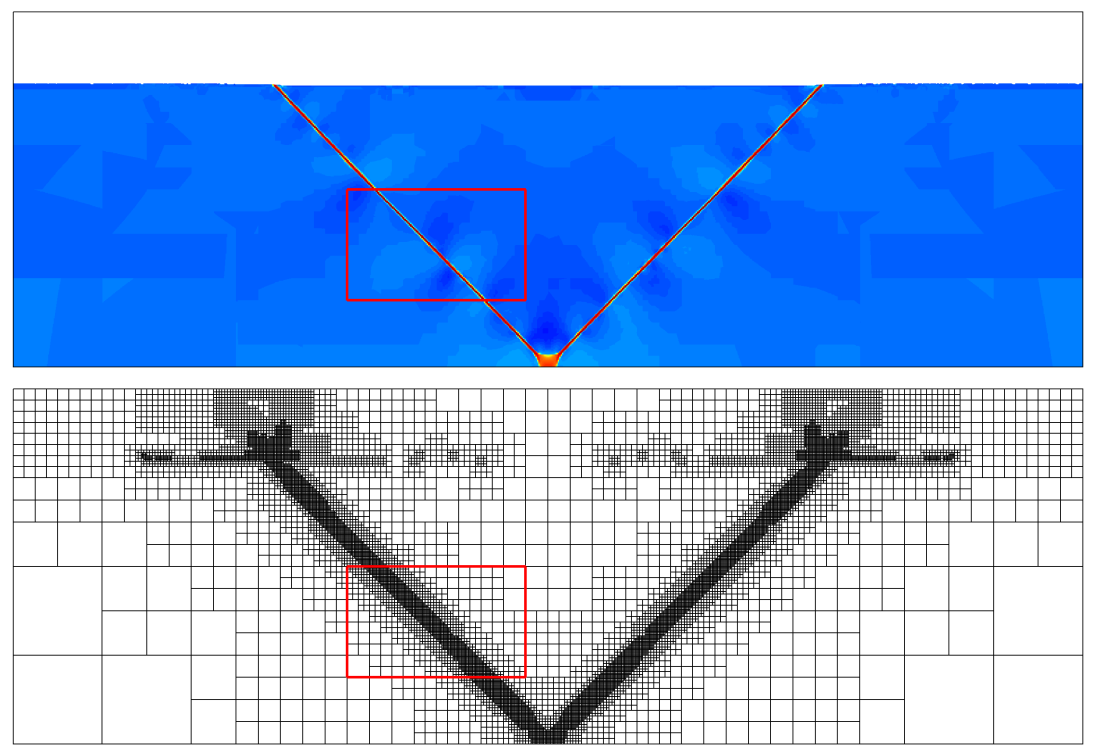
\includegraphics[width=3.74cm]{images/benchmark_brick/mishinb}
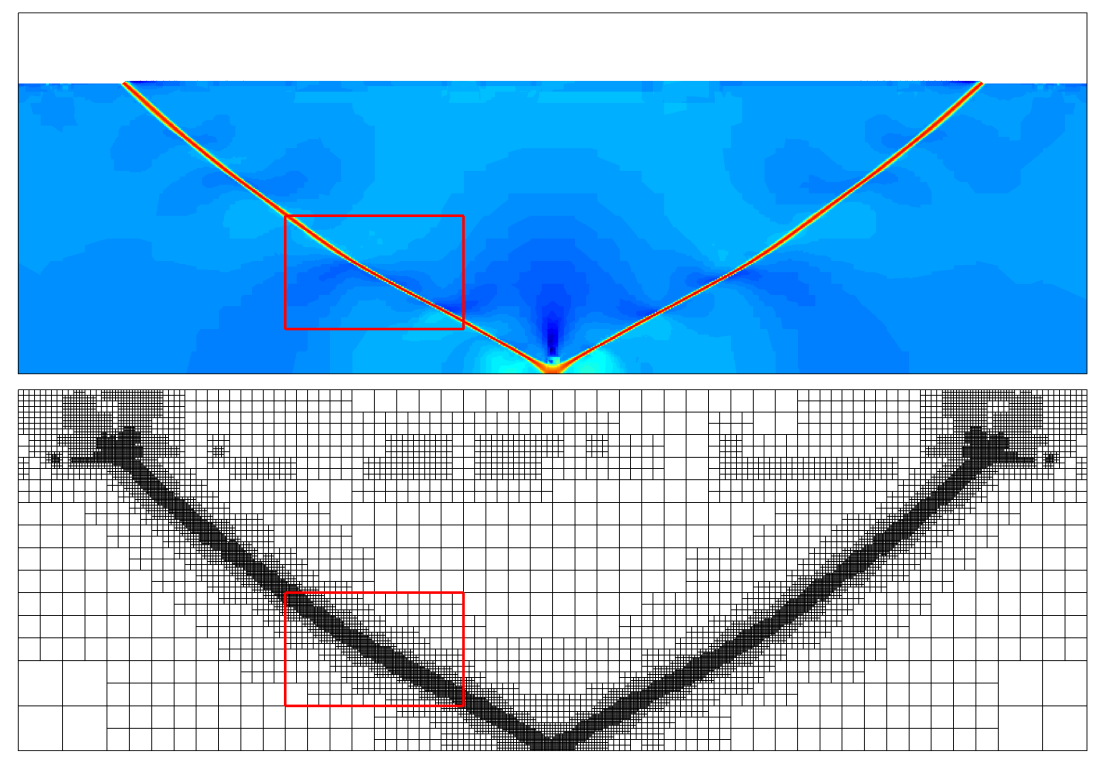
\includegraphics[width=3.74cm]{images/benchmark_brick/mishinc}
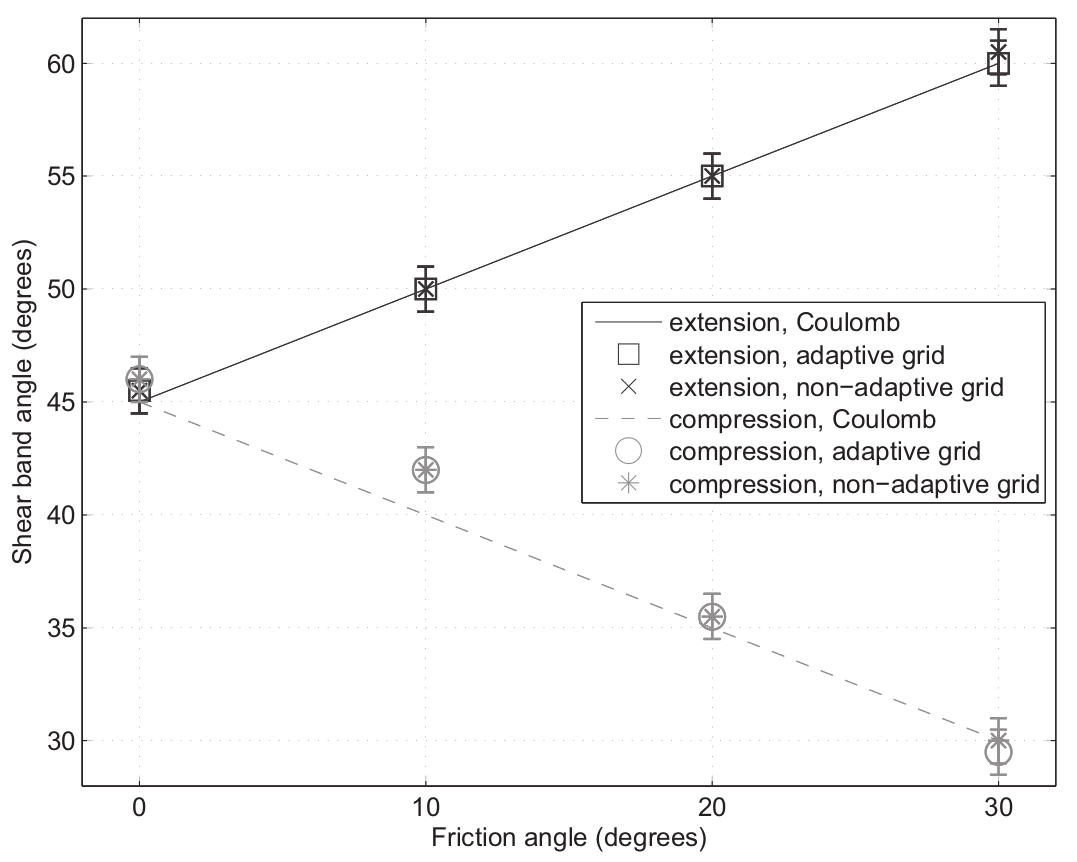
\includegraphics[width=3.74cm]{images/benchmark_brick/mishind}\\
{\small Mishin, phd thesis, 2011 \cite{mishin11}}
\end{center}

\begin{center}\noindent\rule{8cm}{0.4pt}\end{center}

\begin{center}
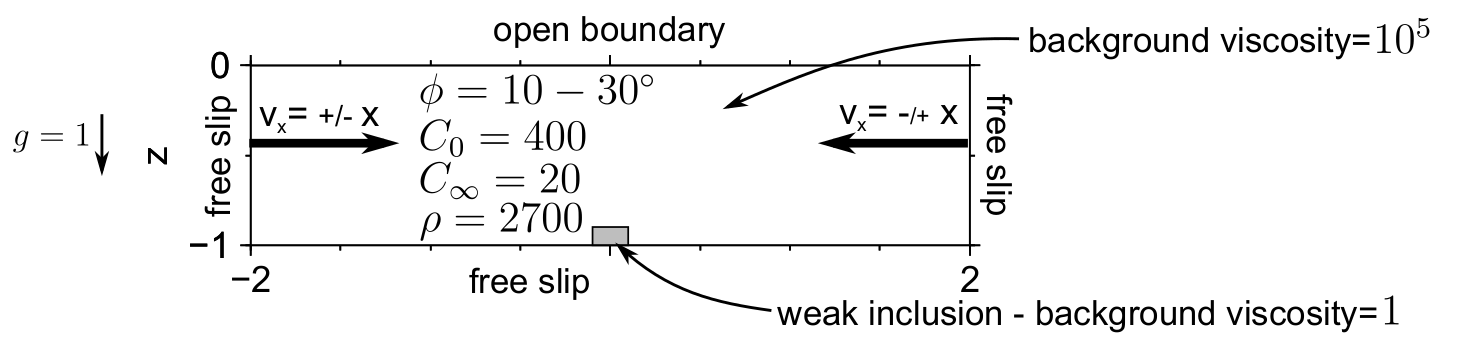
\includegraphics[width=8cm]{images/benchmark_brick/maie12a}
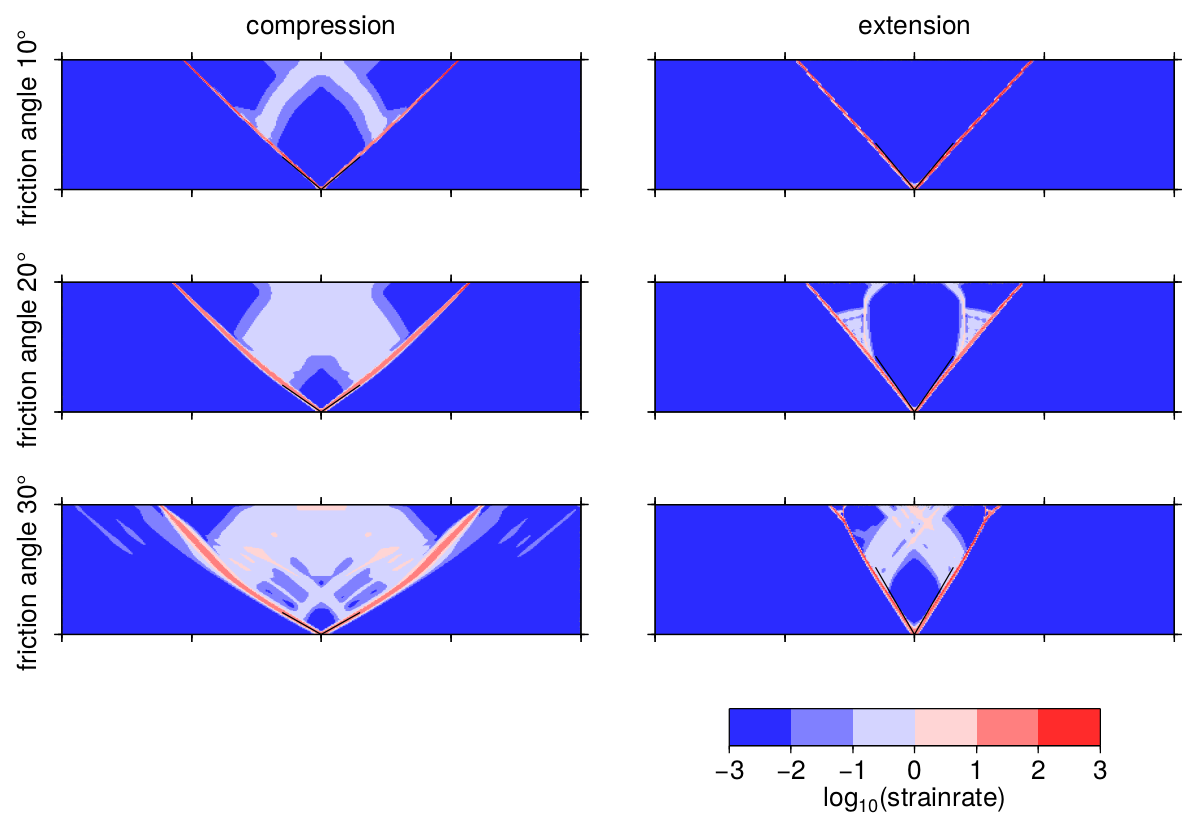
\includegraphics[width=5cm]{images/benchmark_brick/maie12b}\\
{\small Maierova, phd thesis, 2012 \cite{maie12}}
\end{center}

\begin{center}\noindent\rule{8cm}{0.4pt}\end{center}

\begin{center}
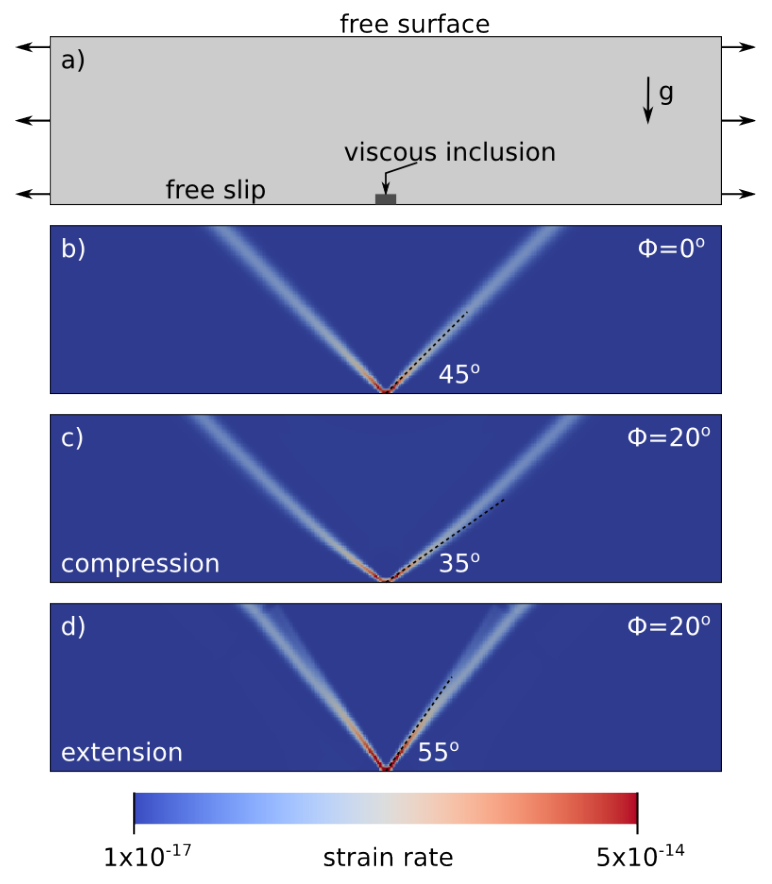
\includegraphics[width=5cm]{images/benchmark_brick/thie14a}
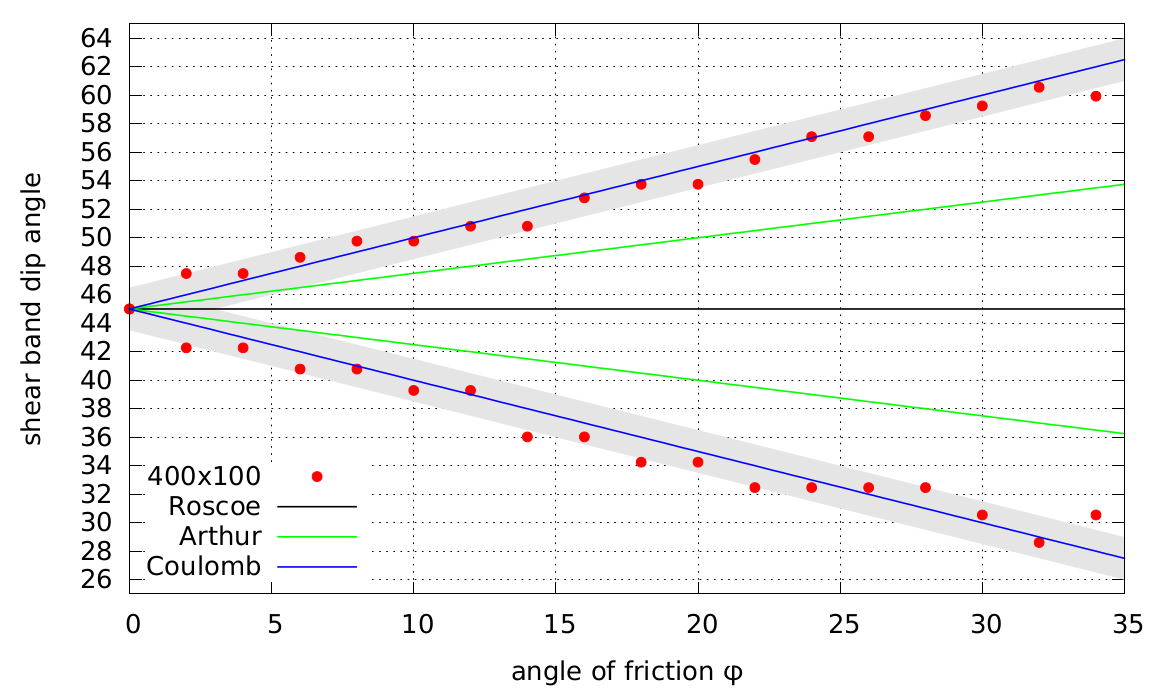
\includegraphics[width=8cm]{images/benchmark_brick/thie14b}\\
{\small Thieulot, 2014 \cite{thie14}}
\end{center}

\begin{center}\noindent\rule{8cm}{0.4pt}\end{center}

\begin{center}
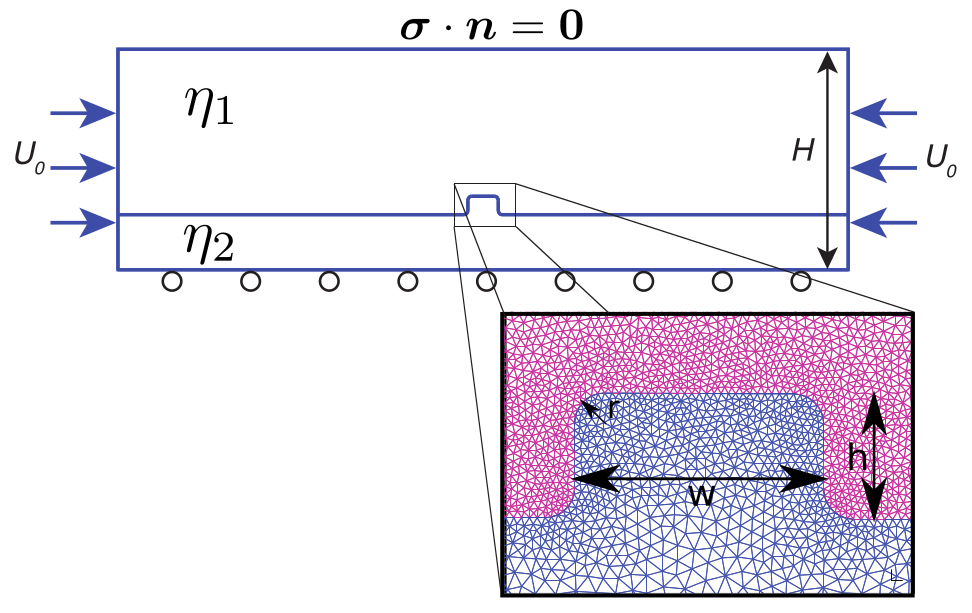
\includegraphics[width=5cm]{images/benchmark_brick/spmw16a}
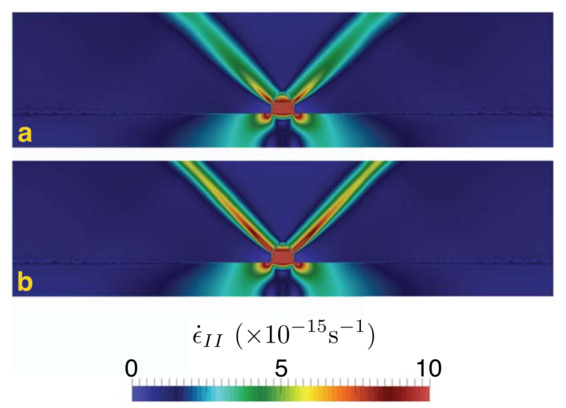
\includegraphics[width=5cm]{images/benchmark_brick/spmw16b}\\
{\small Spiegelman et al, 2016 \cite{spmw16}}
\end{center}

\begin{center}\noindent\rule{8cm}{0.4pt}\end{center}

\begin{center}
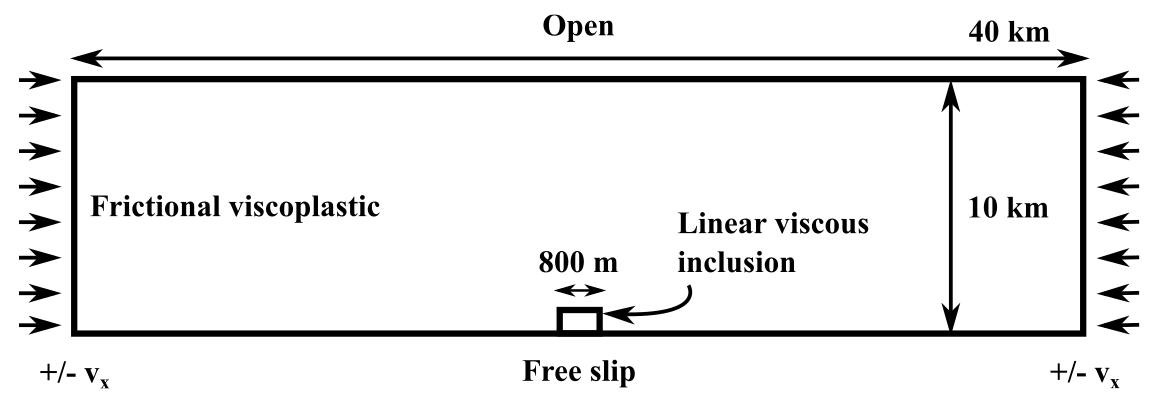
\includegraphics[width=5cm]{images/benchmark_brick/gltf18a}
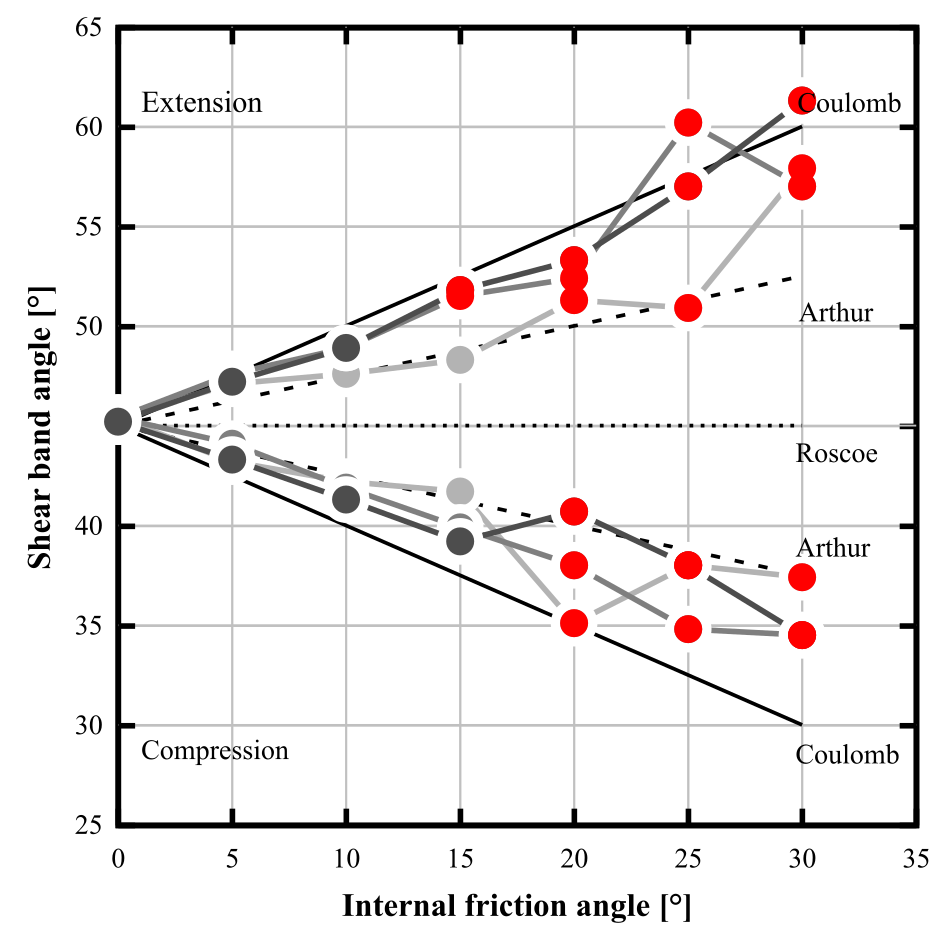
\includegraphics[width=5cm]{images/benchmark_brick/gltf18b}
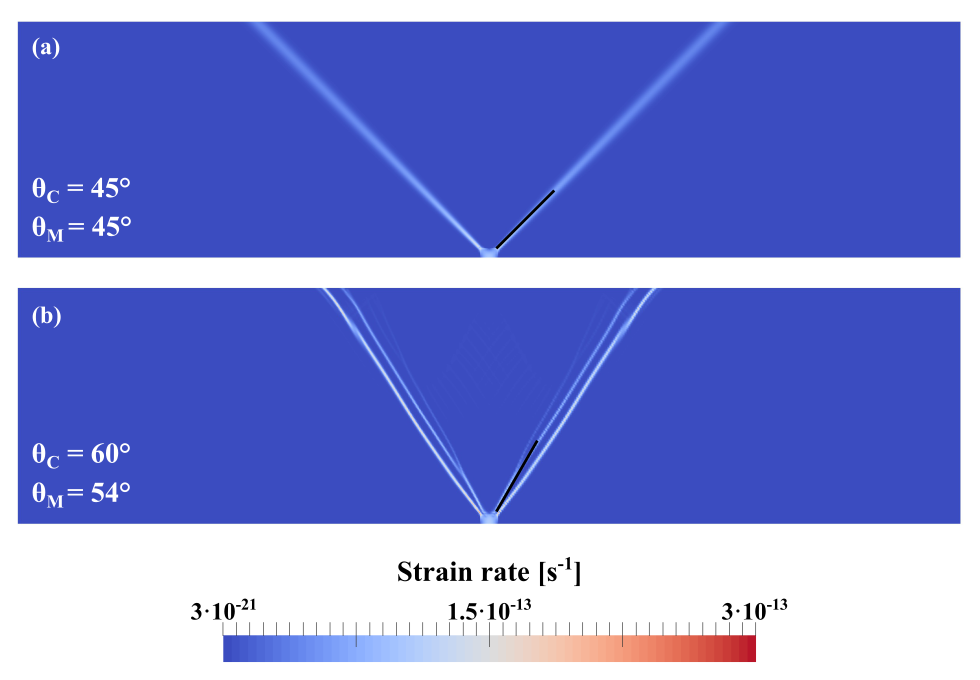
\includegraphics[width=5cm]{images/benchmark_brick/gltf18c}\\
{\small Glerum et al, 2018 \cite{gltf18}}
\end{center}

\begin{center}\noindent\rule{8cm}{0.4pt}\end{center}

\begin{center}
\begin{minipage}{0.45\textwidth}
\centering
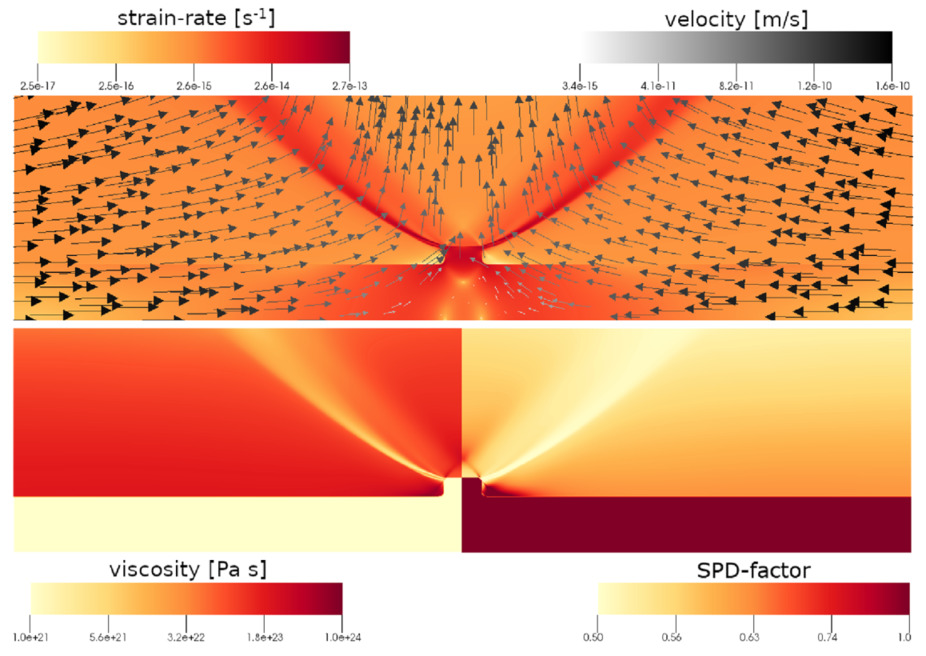
\includegraphics[height=0.8\textwidth]{images/benchmark_brick/frbt19}\\
{\small Fraters et al, 2019 \cite{frbt19}}
\end{minipage}\hfill
\begin{minipage}{0.45\textwidth}
\centering
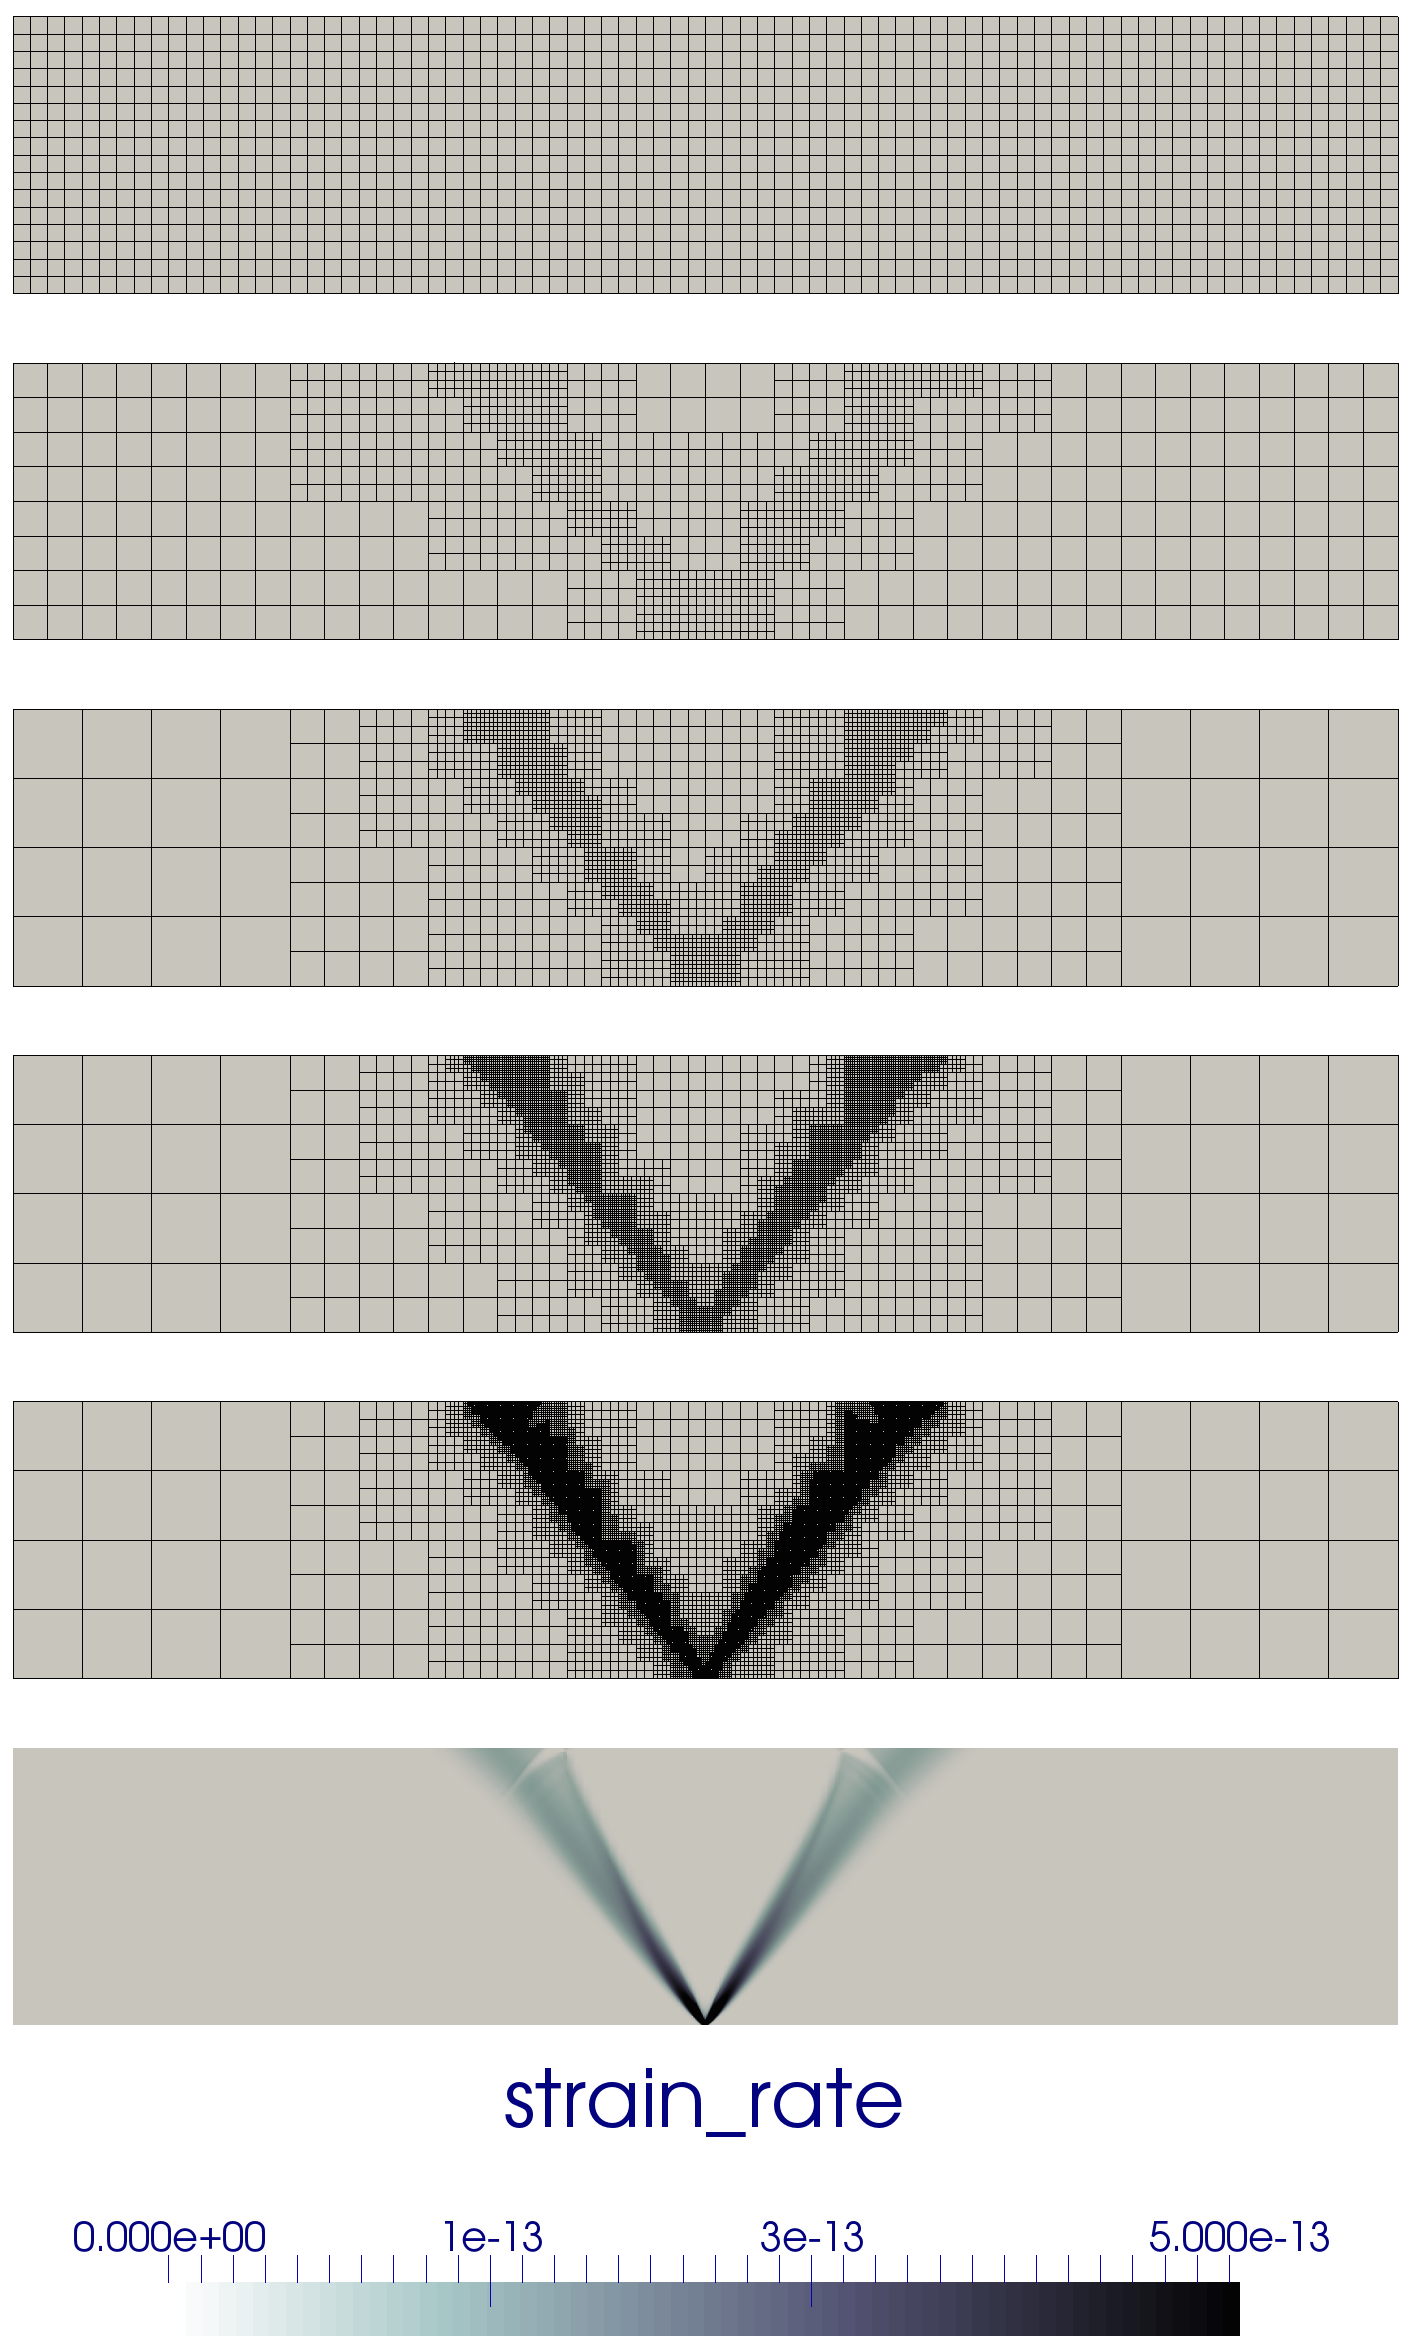
\includegraphics[height=0.8\textwidth]{images/benchmark_brick/aspectmanual}\\
{\small Aspect manual \cite{aspectmanual}}
\end{minipage}
\end{center}
